\section{Monday for MAT4002}\index{Monday_lecture}

\paragraph{Reviewing}
\begin{enumerate}
\item
Topological Space $(X,\mathcal{J})$: a special class of topological space is that induced from metric space $(X,d)$:
\[
(X,\mathcal{T}),\quad\text{with }\mathcal{T}=\{\text{all open sets in $(X,d)$}\}
\]
\item
Closed Sets $(X\setminus U)$ with $U$ open.
\end{enumerate}

\begin{proposition}
Let $(X,\mathcal{T})$ be a topological space, 
\begin{enumerate}
\item
$\emptyset, X$ are closed in $X$
\item
$V_1,V_2$ closed in $X$ implies that $V_1\bigcup V_2$ closed in $X$
\item
$\{V_\alpha\mid\alpha\in\mathcal{A}\}$ closed in $X$ implies that $\bigcap_{\alpha\in\mathcal{A}}V_\alpha$ closed in $X$
\end{enumerate}
\end{proposition}
\begin{proof}
Applying the De Morgan's Law
\[
(X\setminus\bigcup_{i\in I}U_i)=\bigcap_{i\in I}(X\setminus U_i)
\]
\end{proof}

\subsection{Convergence in topological space}

\begin{definition}[Convergence]
A sequence $\{x_n\}$ of a topological space $(X,\mathcal{T})$ converges to $x\in X$ 
if $\forall U\ni x$ is open, there $\exists N$ such that $x_n\in U,\forall n\ge N$.
\end{definition}

\begin{example}
\begin{enumerate}
\item
The topology for the space $(X=\mathbb{R}^n,d_2)\to(X,\mathcal{T})$ (i.e., a topological space induced from meric space $(X=\mathbb{R}^n,d_2)$) is called a \emph{usual topology} on $\mathbb{R}^n$.

When I say $\mathbb{R}^n$ (or subset of $\mathbb{R}^n$) is a topological space, 
it is equipeed with usual topology.

Convergence of sequence in $(\mathbb{R}^n,\mathcal{T})$ is the usual convergence in analysis.

For $\mathbb{R}^n$ or metric space, the limit of sequence (if exists) is unique.

\item

Consider the topological space $(X,\mathcal{T}_{\text{indiscrete}})$. 
Take any sequence $\{x_n\}$ in $X$, it is convergent to any $x\in X$. 
Indeed, for $\forall U\ni x$ open, $U=X$. Therefore, 
\[
x_n\in U(=X),\forall n\ge1.
\]
\item

Consider the topological space $(X,\mathcal{T}_{\text{cofinite}})$, where $X$ is infinite. 
Consider $\{x_n\}$ is a sequence satisfying $m\ne n$ implies $x_m\ne x_n$. 
Then $\{x_n\}$ is convergent to any $x\in X$.

(Question: how to define openness for $\mathcal{T}_{\text{cofinite}}$ and $\mathcal{T}_{\text{indiscrete}})$?
\item

Consider the topological space $(X,\mathcal{T}_{\text{discrete}})$, 
the sequence $\{x_n\}\to x$ is equivalent to say $x_n=x$ for all sufficiently large $n$.
\end{enumerate}
\end{example}
\begin{remark}
The limit of sequences may not be unique. The reason is that ``$\mathcal{T}$ is not big enough''. We will give a criterion to make sure the limit is unique in the future. (Hausdorff)
\end{remark}
\begin{proposition}\label{pro:2:9}
If $F\subseteq(X,\mathcal{T})$ is closed, then for any convergent sequence $\{x_n\}$ in $F$, the limit(s) are also in $F$.
\end{proposition}

\begin{proof}
Let $\{x_n\}$ be a sequence in $F$ with limit $x\in X$. 
Suppose on the contrary that $x\notin F$ 
(i.e., $x\in X\setminus F$ that is open). 
There exists $N$ such that
\[
x_n\in X\setminus F,\forall n\ge N,
\]
i.e., $x_n\notin F$, which is a contradiction.
\end{proof}
\begin{remark}
The converse may not be true. If the $(X,\mathcal{T})$ is metrizable, the converse holds.

Counter-example: Consider the co-countable topological space $(X,\mathcal{T}_{\text{co-co}})$, where 
\[
\mathcal{T}_{\text{co-co}}=
\{U\mid X\setminus U\text{ is a countable set}\}
\bigcup\{\emptyset\},
\]
and $X$ is uncontable. 
Let $F\subsetneqq$ be an un-countable set such that is closed under limits, e.g., $[0,1]$. It's clear that $X\setminus F\notin \mathcal{T}_{\text{co-co}}$, i.e., $F$ is not closed.
\end{remark}

\subsection{Interior, Closure, Boundary}
\begin{definition}\label{def:2:5}
Let $(X,\mathcal{T})$ be a topological space, and $A\subseteq X$ a subset.
\begin{enumerate}
\item
The \emph{interior} of $A$ is 
\[
A^\circ=\bigcup_{U\subseteq A,U\text{ is open}}U
\]
\item
The \emph{closure} of $A$ is
\[
\overline{A}=\bigcap_{A\subseteq V,V\text{ is closed}}V
\]
\end{enumerate}

If $\overline{A}=X$, we say that $A$ is dense in $X$.

The graph illustration of the definition above is as follows:
\begin{figure}[H]
        \begin{subfigure}[b]{0.3\textwidth}
                \centering
                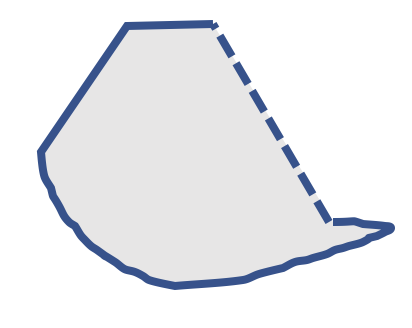
\includegraphics[width=\textwidth]{week2/p_1}
                \caption{Illustration of $A$}
                \label{fig:gull}
        \end{subfigure}%
        \begin{subfigure}[b]{0.3\textwidth}
                \centering
                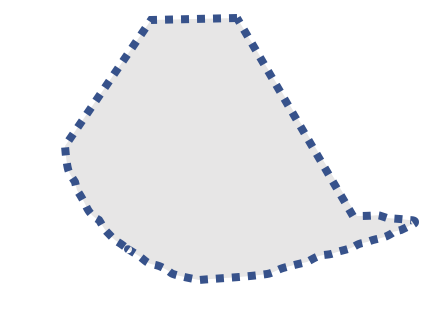
\includegraphics[width=\textwidth]{week2/p_2}
                \caption{Illustration of $A^\circ$}
                \label{fig:gull2}
        \end{subfigure}%
        \begin{subfigure}[b]{0.3\textwidth}
                \centering
                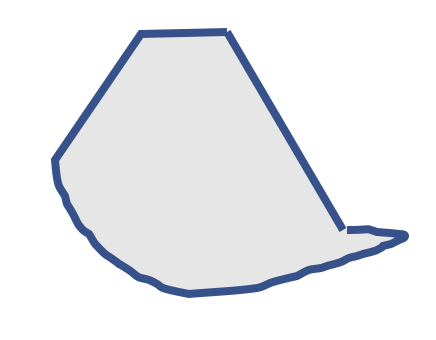
\includegraphics[width=\textwidth]{week2/p_3}
                \caption{Illustration of $\overline{A}$}
                \label{fig:tiger}
        \end{subfigure}
        \caption{Graph Illustrations}\label{fig:animals}
\end{figure}
\end{definition}
\begin{example}
\begin{enumerate}
\item

For $[a,b)\subseteq\mathbb{R}$, we have:
\[
\begin{array}{ll}
[a,b)^\circ=(a,b),
&
\overline{[a,b)}=[a,b]
\end{array}
\]

\item
For $X=\mathbb{R}$, $\mathbb{Q}^\circ=\emptyset$ and $\overline{\mathbb{Q}}=\mathbb{R}$.

\item
Consider the discrete topology $(X,\mathcal{T}_{\text{discrete}})$, we have
\[
\begin{array}{ll}
S^\circ=S,
&
\overline{S}=S
\end{array}
\]

\end{enumerate}
\end{example}

The insights behind the definition~(\ref{def:2:5}) is as follows

\begin{proposition}
\begin{enumerate}
\item
$A^\circ$ is the largest open subset of $X$ contained in $A$;

$\overline{A}$ is the smallest closed subset of $X$ containing $A$.
\item
If $A\subseteq B$, then $A^\circ\subseteq B$ and $\overline{A}\subseteq\overline{B}$
\item
$A$ is open in $X$ is equivalent to say $A^\circ = A$; $A$ is closed in $X$ is equivalent to say $\overline{A}=A$.
\end{enumerate}
\end{proposition}

\begin{example}
Let $(X,d)$ be a metric space. What's the closure of an open ball $B_r(x)$?

The direct intuition is to define the closed ball
\[
\bar B_r(x)=\{y\in X\mid d(x,y)\le r\}.
\]

Question: is $\bar B_r(x)=\overline{B_r(x)}$?
\begin{enumerate}
\item
Since $\bar B_r(x)$ is a closed subset of $X$, and 
$B_r(x)\subseteq \bar B_r(x)$, 
we imply that
\[
\overline{B_r(x)}\subseteq\bar B_r(x)
\]
\item
Howover, we may find an example such that $\overline{B_r(x)}$ is a proper subset of $\bar B_r(x)$:

Consider the discrete metric space $(X,d_{\text{discrete}})$ and for $\forall x\in X$,
\[
B_1(x)=\{x\}\implies
\overline{B_1(x)}=\{x\},\quad
\bar B_1(x)=X
\]

The equality $\bar B_r(x)=\overline{B_r(x)}$ holds when $(X,d)$ is a normed space.
\end{enumerate}
\end{example}

Here is another characterization of $\overline{A}$:

\begin{proposition}
\[
\overline{A}=\{x\in X\mid\forall \text{open }U\ni x, U\bigcap A\ne\emptyset\}
\]
\end{proposition}
\begin{proof}
Define
\[
S=\{x\in X\mid\forall \text{open }U\ni x, U\bigcap A\ne\emptyset\}
\]
It suffices to show that $\overline{A}=S$.
\begin{enumerate}
\item
First show that $S$ is closed:
\[
X\setminus S=\{x\in X\mid\exists U_x\ni x\text{ open s.t. }U_x\bigcap A=\emptyset\}
\]
Take $x\in X\setminus S$, we imply there exists open $U_x\ni x$ such that $U_x\bigcap A=\emptyset$. We claim $U_x\subseteq X\setminus S$:
\begin{itemize}
\item
For $\forall y\in U_x$, note that $U_x\ni y$ that is open, such that $U_x\bigcap A=\emptyset$. Therefore, $y\in X\setminus S$.
\end{itemize}

Therefore, we have $x\in U_x\subseteq X\setminus S$ for any $\forall x\in X\setminus S$.

Note that
\[
X\setminus S
=
\bigcup_{x\in X\setminus S}\{x\}\subseteq
\bigcup_{x\in X\setminus S}U_x\subseteq X\setminus S,
\]
which implies $X\setminus S=\bigcup_{x\in X\setminus S}U_x$ is open, i.e., $S$ is closed in $X$.
\item
By definition, it is clear that $A\subseteq S$:
\[
\forall a\in A,\forall\text{open }U\ni a,
U\bigcap A\supseteq\{a\}\ne\emptyset\implies a\in S.
\]
Therefore, $\overline{A}\subseteq\overline{S}=S$.
\item
Suppose on the contrary that 
there exists $y\in S\setminus\overline{A}$. 

Since $y\notin\overline{A}$, by definition, 
there exists $F\supseteq A$ closed such that 
$y\notin F$. 

Therefore, $y\in X\setminus F$ that is open, and 
\[
(X\setminus F)\bigcap A\subseteq(X\setminus A)\bigcap A=\emptyset\implies y\notin S,
\]
which is a contradiction. Therefore, $S=\overline{A}$.
\end{enumerate}
\end{proof}
\begin{definition}[accumulation point]
Let $A\subseteq X$ be a subset in a topological space. 
We call $x\in X$ are an 
\emph{accumulation point} (\emph{limit point}) of $A$ 
if
\[
\forall U\subseteq X\text{ open s.t. }
U\ni x, 
(U\setminus\{x\})\bigcap A\ne\emptyset.
\]

The set of accumulation points of $A$ is denoted as $A'$
\end{definition}
\begin{proposition}
$\overline{A}=A\bigcup A'$.
\end{proposition}











